\documentclass[../notes.tex]{subfiles}

\pagestyle{main}
\renewcommand{\chaptermark}[1]{\markboth{\chaptername\ \thechapter\ (#1)}{}}
\setcounter{chapter}{5}

\begin{document}




\chapter{Complex MO Diagrams}
\section{MO Theory: LCAOs and Group Orbitals}
\begin{itemize}
    \item \marginnote{10/31:}Last time: Building MO diagrams by qualitatively identifying a basis of atomic orbitals (e.g., 1s for H, 2s and 2p for F) and intuitively determining an axis to about which they transform within the linear point group $C_{\infty v}$.
    \item Today: Making this process more formal, as is necessary for more complex, polyatomic molecules.
    \item For polyatomic molecules, we need to determine how the basis atomic orbitals transform. This will allow us to approximate molecular orbitals with linear combinations of them (the AOs) that transform with the same symmetry.
    \begin{itemize}
        \item To do this, we need to understand how to group together valence atomic orbitals, i.e., how to construct \textbf{group orbitals}.
    \end{itemize}
    \item \textbf{Group orbital}: An MO of a complex molecule.
    \item Strategy for building group orbitals and creating the relevant MO diagram.
    \begin{enumerate}
        \item Determine the point group of the molecule. If it is a linear molecule, substituting a simpler point group that still retains the symmetry of the orbitals (ignoring the signs) makes the process easier by eliminating infinite-fold rotation axes.
        \begin{itemize}
            \item We will substitute the 2-fold \textbf{subgroup} of the relevant point group in these cases.
            \item In particular, substitute $D_{2h}$ for $D_{\infty h}$ and $C_{2v}$ for $C_{\infty v}$.
        \end{itemize}
        \item Assign $xyz$ coordinates.
        \item Construct reducible representations for the valence orbitals on the peripheral atoms.
        \item Reduce each representation to its IRRs (i.e., find the symmetry of the group orbitals). Group orbitals are the combinations of atomic orbitals that match the symmetry of the IRRs.
        \item Identify the atomic orbitals on the central atom with the same symmetries (IRRs) as those found in step 4.
        \item Combine the atomic orbitals with matching symmetry and similar energy. The total number of MOs must be equal to the number of atomic orbitals used from all the atoms.
        \begin{itemize}
            \item Energy scaling of MOs $\sigma<\pi<\text{lone pairs}<\pi^*<\sigma^*$. More nodes equals higher in energy.
        \end{itemize}
        \item Label MOs.
        \begin{itemize}
            \item $\sigma$ implies a SALC with infinite-fold rotational symmetry about the bond axis; $\pi$ implies a SALC with 2-fold rotational symmetry about the bond axis.
            \item No superscript implies a bonding interaction; superscript $*$ implies an antibonding interaction.
            \item Subscript $g$ implies symmetrical with respect to inversion; subscript $u$ implies asymmetrical with respect to inversion.
        \end{itemize}
        \item Fill in the electrons.
    \end{enumerate}
    \item Example: \ce{CO2}.
    \begin{enumerate}
        \item $D_{\infty h}\to D_{2h}$.
        \begin{table}[h!]
            \centering
            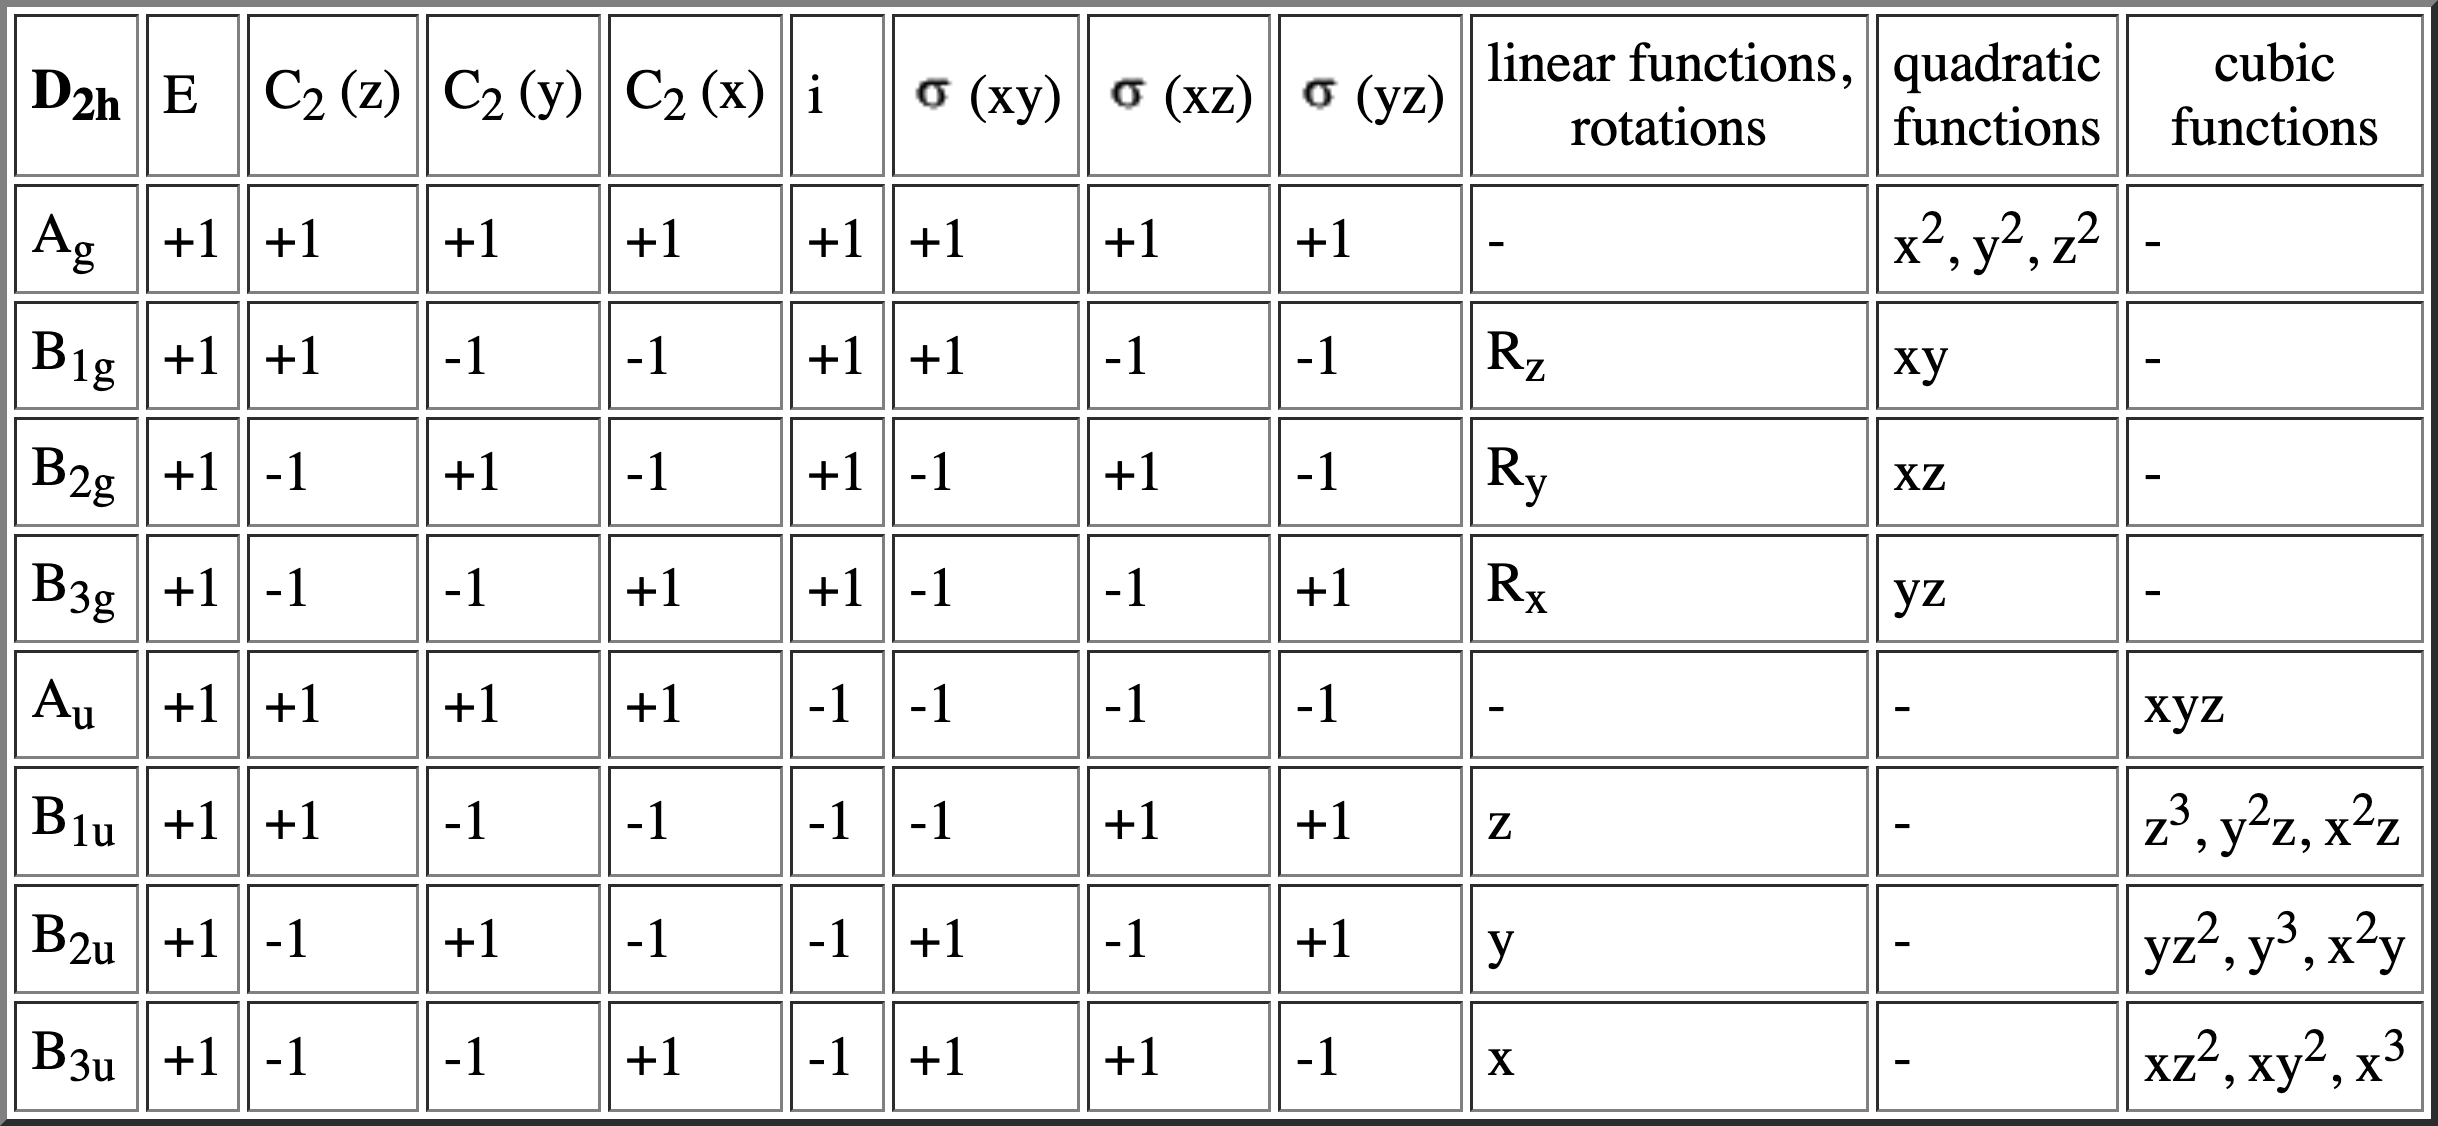
\includegraphics[width=0.8\linewidth]{../ExtFiles/charTableD2h.png}
            \caption{$D_{2h}$ character table.}
            \label{tab:charTableD2h}
        \end{table}
        \item $xyz$ coordinates are chosen as per Figure \ref{fig:CO2xyz}.
        \begin{figure}[h!]
            \centering
            \footnotesize
            \begin{tikzpicture}
                \node{
                    \chemfig{O=@{C}C=@{O}O}
                    \chemmove{
                        \draw [-latex,shorten <=2pt] (O) -- ++(0.7,0,0) node[right]{$z$};
                        \draw [-latex,shorten <=2pt] (C) -- ++(0,0.7,0) node[above]{$x$};
                        \draw [-latex,shorten <=2pt] (C) -- ++(0,0,1.2) node[below left=-2pt]{$y$};
                    }
                };
                \path (-1.1,-0.75) rectangle (1.85,1);
            \end{tikzpicture}
            \caption{\ce{CO2} $xyz$ coordinates.}
            \label{fig:CO2xyz}
        \end{figure}
        \item The two oxygen atoms are peripheral; their valence orbitals are $2s$, $2p_x$, $2p_y$, and $2p_z$. Thus, we have from the $D_{2h}$ character table and Figure \ref{fig:CO2xyz} that
        \begin{table}[h!]
            \centering
            \small
            \renewcommand{\arraystretch}{1.2}
            \begin{tabular}{c|cccccccc}
                $D_{2h}$ & $E$ & $C_2(z)$ & $C_2(y)$ & $C_2(x)$ & $i$ & $\sigma(xy)$ & $\sigma(xz)$ & $\sigma(yz)$\\
                \hline
                $\Gamma_{\ce{O}(2s)}$ & 2 & 2 & 0 & 0 & 0 & 0 & 2 & 2\\
                $\Gamma_{\ce{O}(2p_z)}$ & 2 & 2 & 0 & 0 & 0 & 0 & 2 & 2\\
                $\Gamma_{\ce{O}(2p_x)}$ & 2 & $-2$ & 0 & 0 & 0 & 0 & 2 & $-2$\\
                $\Gamma_{\ce{O}(2p_y)}$ & 2 & $-2$ & 0 & 0 & 0 & 0 & $-2$ & 2\\
            \end{tabular}
            \caption{Representations for the valence orbitals of \ce{CO2}.}
            \label{tab:CO2RR}
        \end{table}
        \begin{itemize}
            \item We get 0 characters for $\Gamma_{\ce{O}(2p_z)}$ because the individual orbitals move, even though the "overall basis" inverts.
        \end{itemize}
        \item As follows.
        \begin{align*}
            \Gamma_{\ce{O}(2s)} = \Gamma_{\ce{O}(2p_z)} &= a_g+b_{1u}\\
            \Gamma_{\ce{O}(2p_x)} &= b_{3u}+b_{2g}\\
            \Gamma_{\ce{O}(2p_y)} &= b_{2u}+b_{3g}
        \end{align*}
        \item Carbon AOs: From the $D_{2h}$ character table,
        \begin{align*}
            \ce{C}(2s) &= a_g&
            \ce{C}(2p_z) &= b_{1u}&
            \ce{C}(2p_x) &= b_{3u}&
            \ce{C}(2p_y) &= b_{2u}
        \end{align*}
        \item We can now construct the following MO diagram.
        \begin{figure}[H]
            \centering
            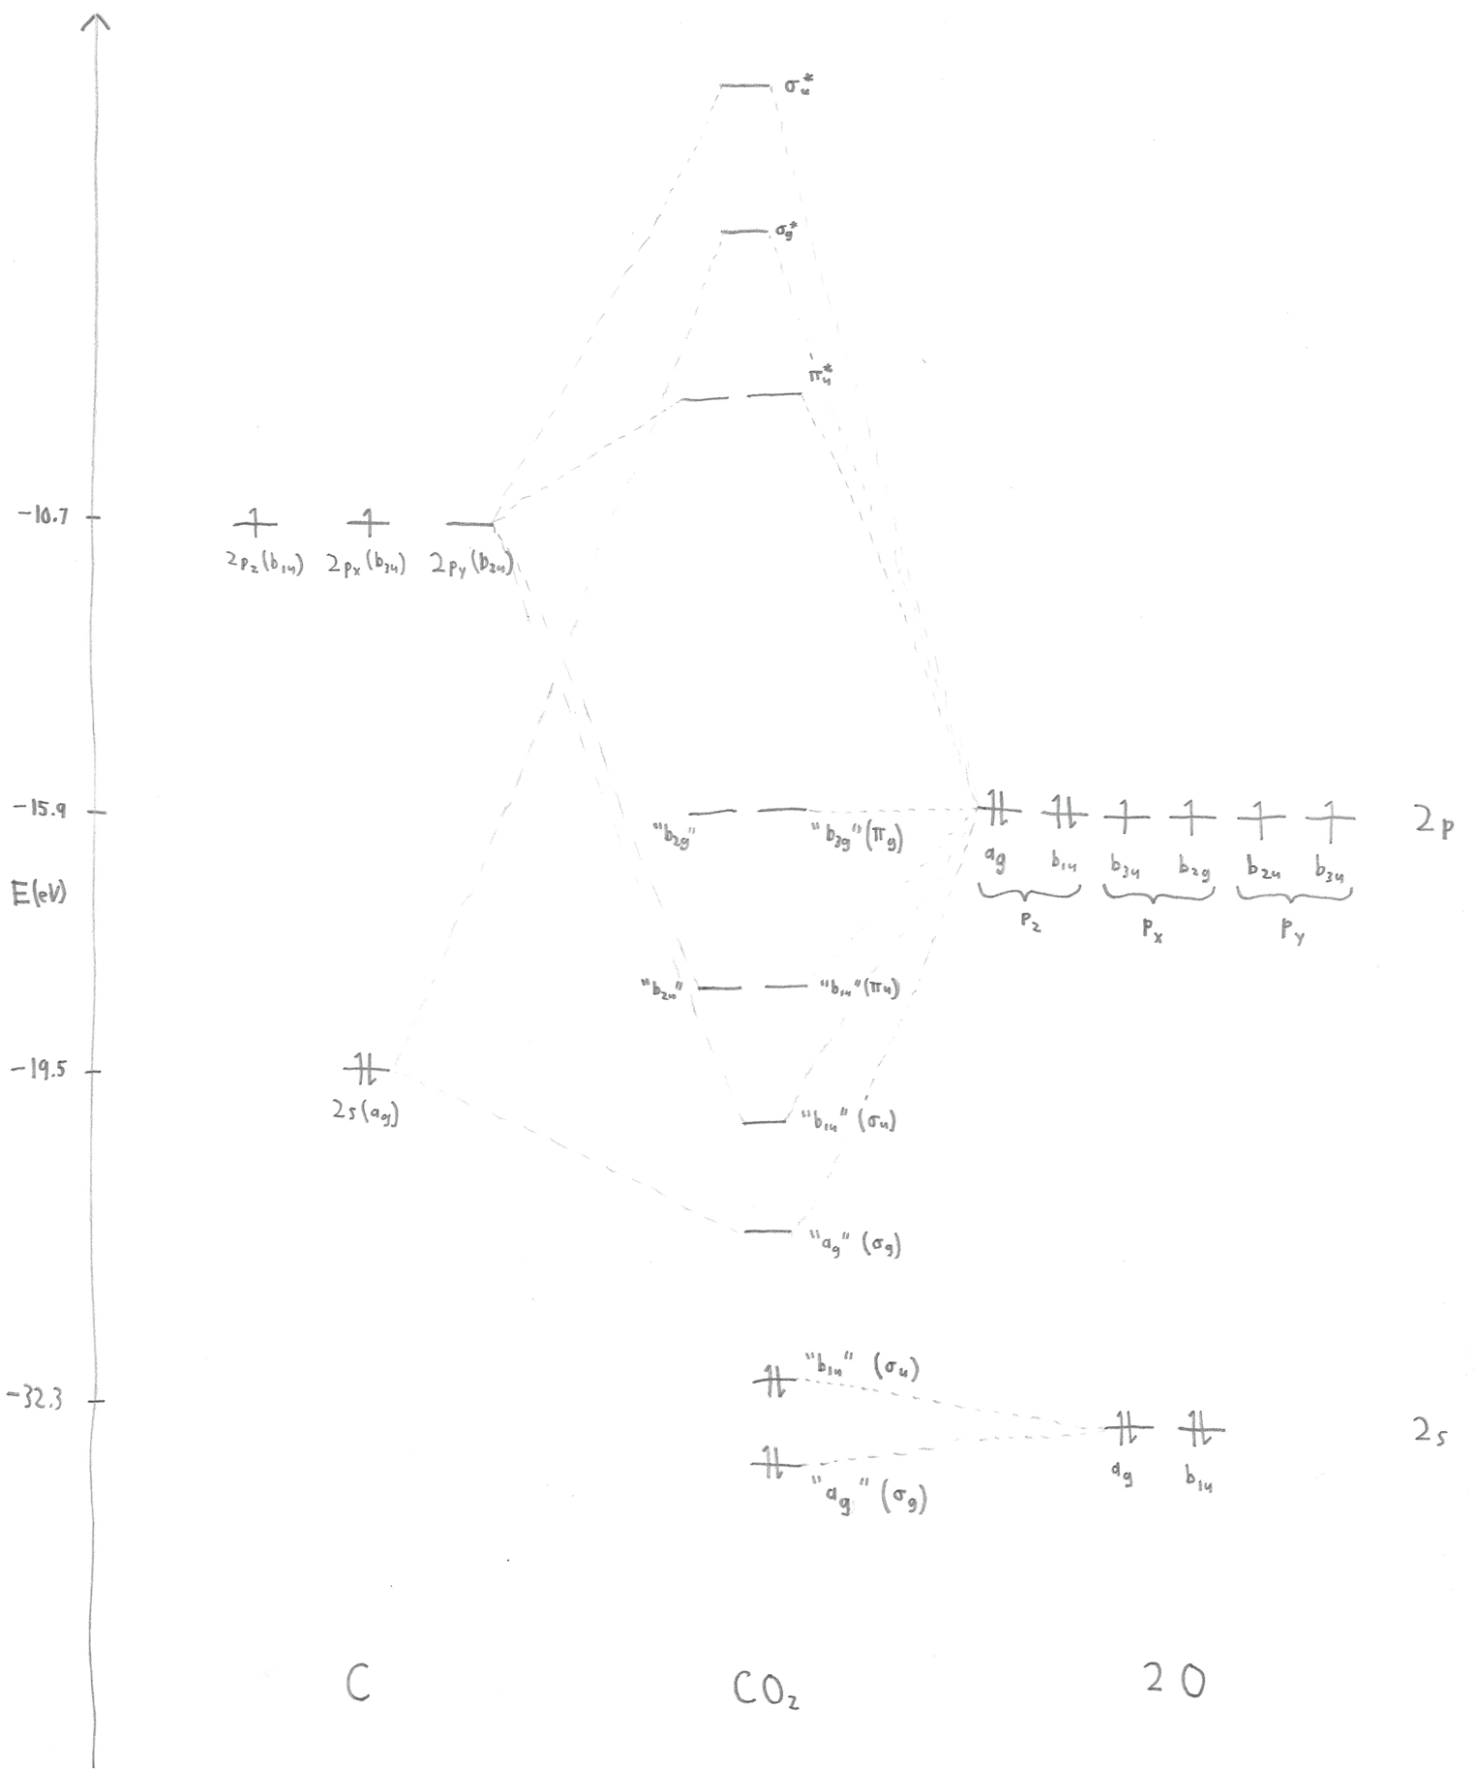
\includegraphics[width=0.7\linewidth]{../ExtFiles/MOsCO2.png}
            \caption{\ce{CO2} MO diagram.}
            \label{fig:MOsCO2}
        \end{figure}
        Moreover, a selection of key SALCs may be visualized as follows.
        \begin{figure}[H]
            \centering
            \begin{subfigure}[b]{0.49\linewidth}
                \centering
                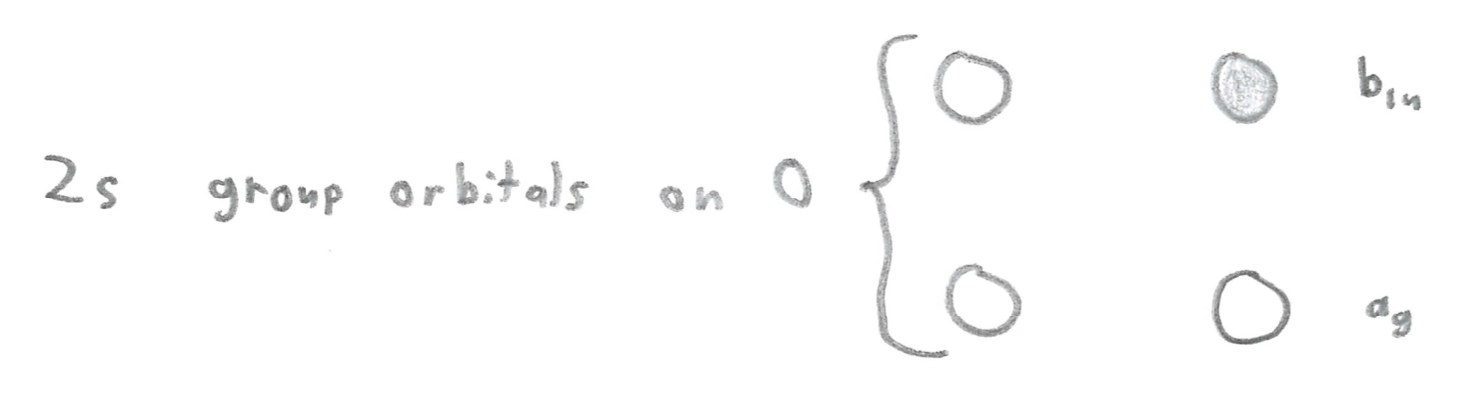
\includegraphics[width=0.8\linewidth]{../ExtFiles/CO2SALCa.png}
                \caption{$\ce{O}(2s)$.}
                \label{fig:CO2SALCa}
            \end{subfigure}
            \begin{subfigure}[b]{0.49\linewidth}
                \centering
                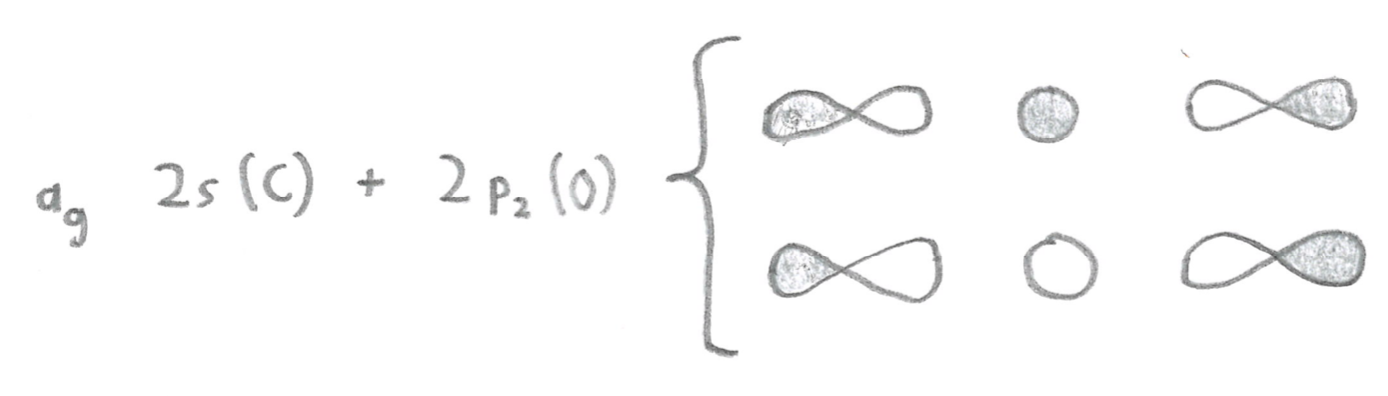
\includegraphics[width=0.8\linewidth]{../ExtFiles/CO2SALCb.png}
                \caption{$a_g$.}
                \label{fig:CO2SALCb}
            \end{subfigure}
        \end{figure}
        \begin{figure}[H]
            \ContinuedFloat
            \centering
            \begin{subfigure}[b]{0.49\linewidth}
                \centering
                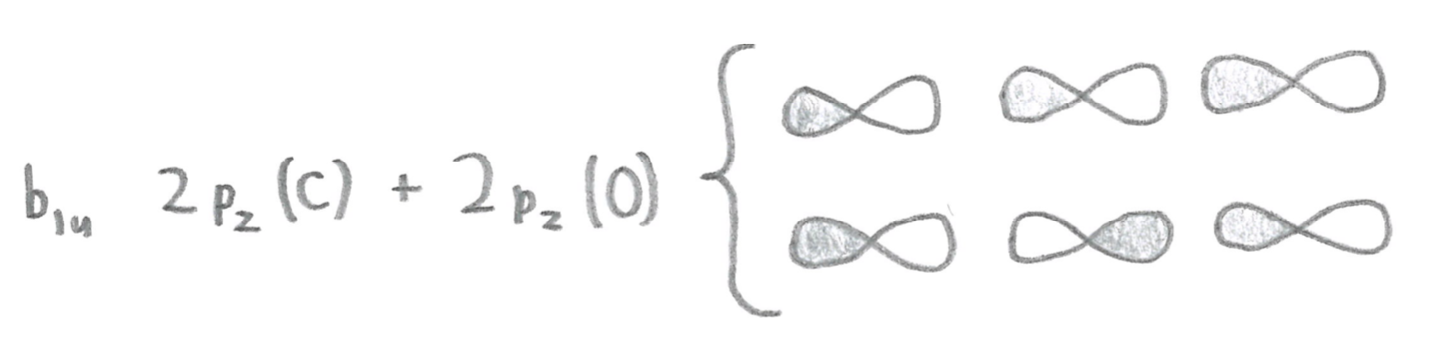
\includegraphics[width=0.8\linewidth]{../ExtFiles/CO2SALCc.png}
                \caption{$b_{1u}$.}
                \label{fig:CO2SALCc}
            \end{subfigure}
            \begin{subfigure}[b]{0.49\linewidth}
                \centering
                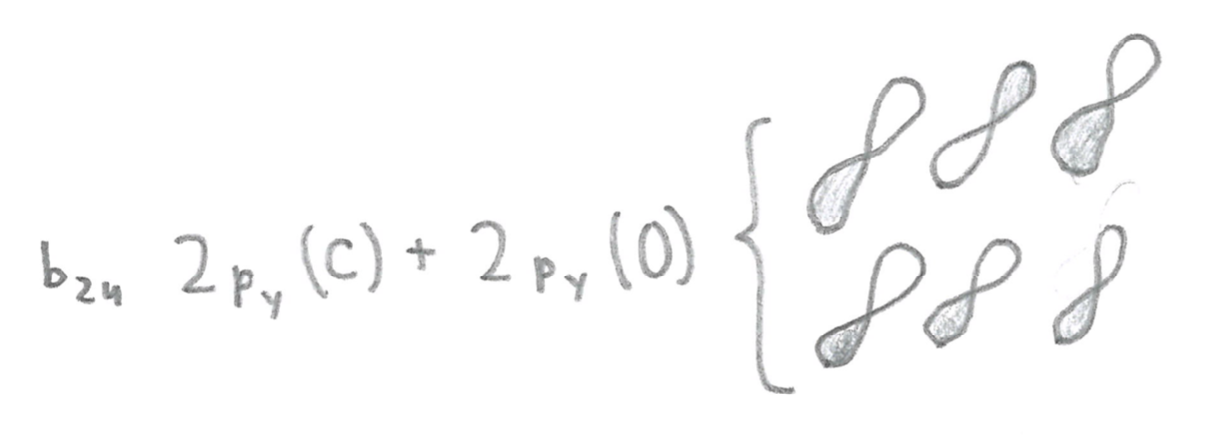
\includegraphics[width=0.8\linewidth]{../ExtFiles/CO2SALCd.png}
                \caption{$b_{2u}$.}
                \label{fig:CO2SALCd}
            \end{subfigure}
            \caption{Selected \ce{CO2} SALCs.}
            \label{fig:CO2SALC}
        \end{figure}
        \begin{itemize}
            \item From the 1 Rydberg rule, oxygen $2s$ orbitals will not significantly overlap with carbon $2s$ or $2p$ orbitals.
            \begin{itemize}
                \item However, we still know that the bonding orbital is slightly lower in energy than the antibonding orbital by counting nodes
                \item A bit of mixing also occurs, though (see the discussion surrounding Figure \ref{fig:calculatedMOsCO2}).
            \end{itemize}
            \item We have so many oxygen electrons since we have \emph{two} oxygens and we are considering their \emph{group} orbitals.
            \item We can draw SALCs intuitively by combining orbitals in a bonding or antibonding fashion, or rigorously using the projection operator.
            \item \emph{Redraw \& add electrons later!}
        \end{itemize}
        \item Done (see Figure \ref{fig:MOsCO2}).
        \item Done (see Figure \ref{fig:MOsCO2}).
    \end{enumerate}
    \item Differences between the \ce{CO2} MOs derived from first principles (Figure \ref{fig:MOsCO2}) and the MOs calculated by a computer's quantum mechanics program (Figure \ref{fig:calculatedMOsCO2}).
    \begin{figure}[H]
        \centering
        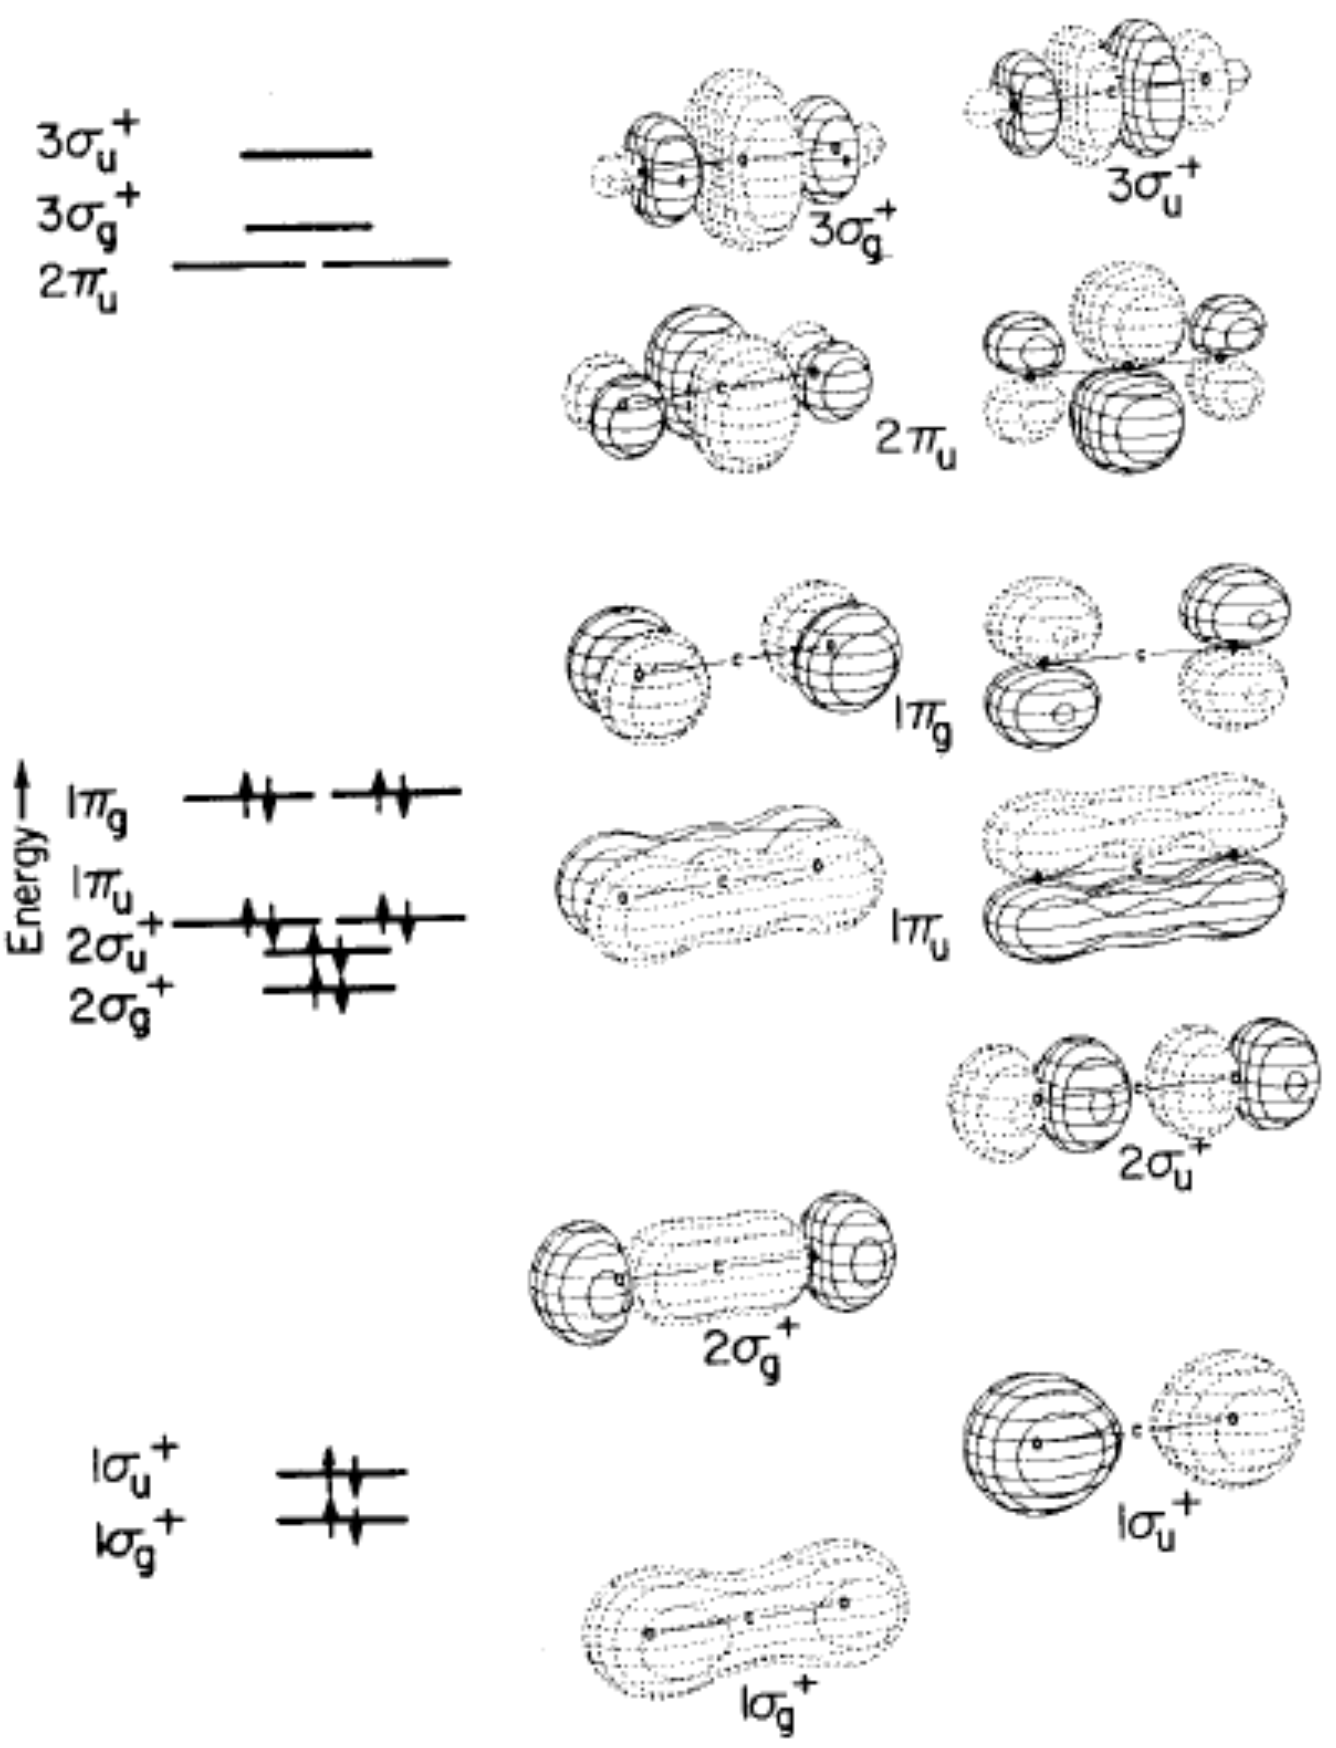
\includegraphics[width=0.5\linewidth]{../ExtFiles/calculatedMOsCO2.png}
        \caption{Quantum-mechanically calculated MOs for \ce{CO2}.}
        \label{fig:calculatedMOsCO2}
    \end{figure}
    \begin{itemize}
        \item In the calculated version, $1\sigma_g$ does not have a node at the carbon atom. This differs from the corresponding SALC we derived from first principles. Thus, in reality, we have some mixing between $1\sigma_g$ and $2\sigma_g$. It follows that we can describe the orbital a bit better as $\ce{O}(2s)$ lone pairs plus \ce{CO} $\sigma$ bonds.
        \item Takeaway: The MOs we get from first principles do not take into account all of the interactions that the computer can.
        \item Note that in Figure \ref{fig:calculatedMOsCO2}, the electron density at each contour surface is \SI[per-mode=symbol]{0.0675}{electrons\per\cubic\angstrom} for one-electron wave functions. This value was chosen merely for satisfactory visual display of the orbitals.
    \end{itemize}
\end{itemize}




\end{document}